  	
\documentclass[tikz]{standalone}
\usepackage[utf8]{inputenc}
\usepackage{tikz}

\begin{document}

    \begin{tikzpicture}		
  		\matrix
  		{
  			\node [text width=9.5cm]{\emph{Resistors} obey Ohm's law: $V=iR$. Through hole resistors are cylindrical with two axial leads and coloured bands that indicate the resistance in ohms.};&
  			\node {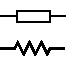
\includegraphics[width=1.2cm]{res-sym}};&
  			\node {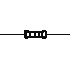
\includegraphics[width=1.2cm]{resistor}};\\
  			
  			\node [text width=9.5cm]{\emph{Capacitors} obey the law $C=Q/V$. The type used in this lab are \emph{multilayer ceramic} capacitors with two parallel leads and a coded capacitance written on the side.};&
  			\node {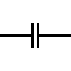
\includegraphics[width=1.2cm]{cap-sym}};&
  			\node {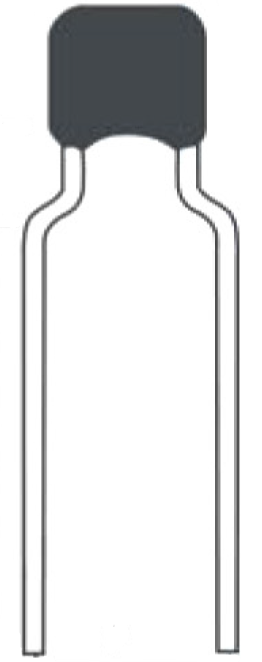
\includegraphics[height=1.2cm]{cap}};\\
  			
  			\node [text width=9.5cm]{The SFH300-3/4 \emph{Phototransistor} conducts a current proportional to the irradiance of visible light and infrared radiation on the sensor. Look for the flat edge on the case flange to identify the collector.};&
  			\node {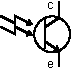
\includegraphics[width=1.2cm]{photoNPN}};&
  			\node {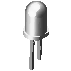
\includegraphics[width=1.2cm]{T13-4}};\\
  			
  			\node [text width=9.5cm]{A \emph{potentiometer} is an adjustable, three-terminal resistor. The resistance between the centre terminal and either end terminal is changed by rotating the shaft.};&
  			\node {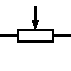
\includegraphics[width=1.2cm]{pot-symbol}};&
  			\node {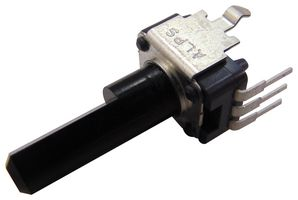
\includegraphics[width=1.2cm]{alps-pot}};\\
  		};
  	\end{tikzpicture}
    \end{document}
